\chapter{Cloud Computing, Orchestrazione e Sicurezza}

\section{Il Modello Cloud Computing}
\begin{figure}[H]
    \centering
    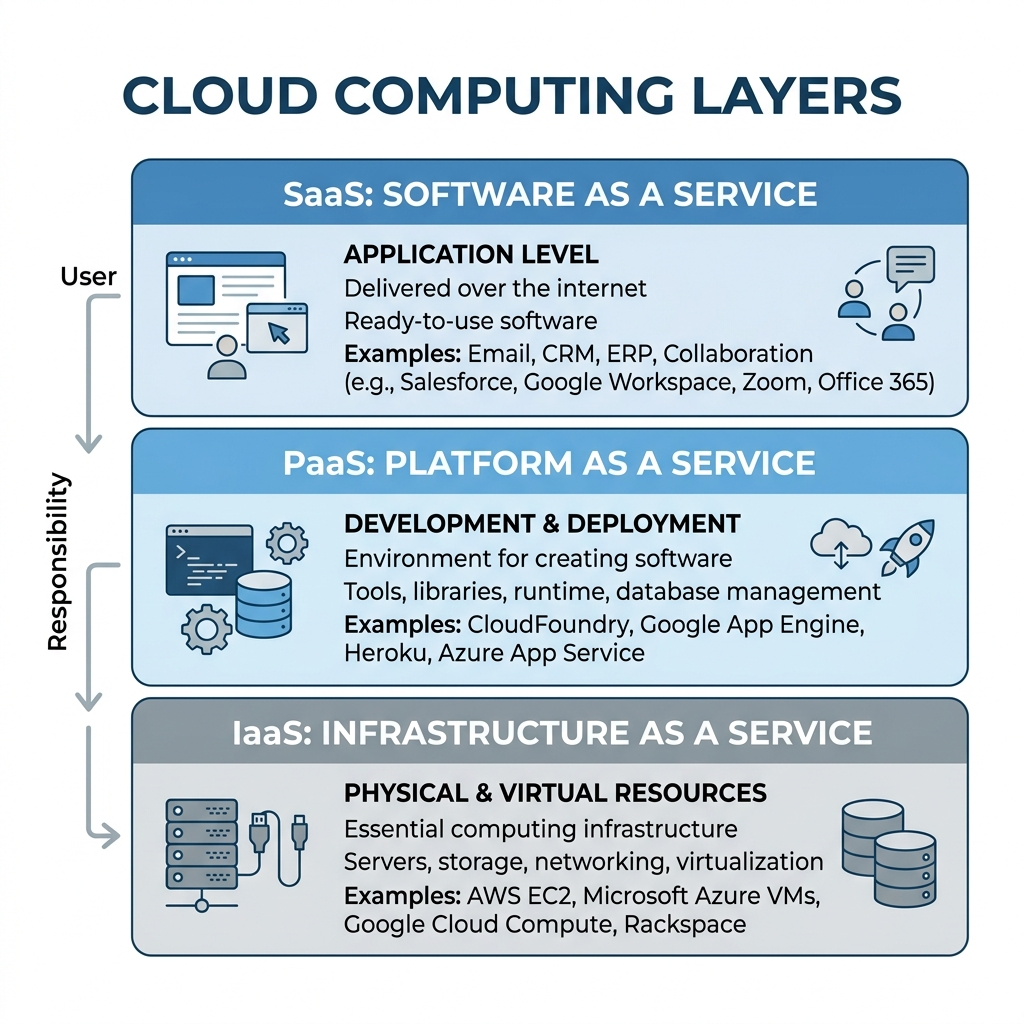
\includegraphics[width=0.8\textwidth]{images/cloud_computing.png}
    \caption{Rappresentazione astratta dei layer dell'architettura Cloud Computing.}
\end{figure}
Il cloud computing rappresenta non solo un cambio tecnologico, ma un profondo mutamento nel modello di business IT: si passa dall'acquisto di hardware (CapEx) al pagamento per consumo di un servizio (OpEx).

\begin{tipbox}[Le Sfide della Pubblica Amministrazione]
Costruire un cloud per un'azienda nativa digitale o per la Pubblica Amministrazione (PA) sono due sfide opposte. Una startup opera in ambiente \textbf{Greenfield} (si parte da zero con standard moderni). La PA opera tipicamente in \textbf{Brownfield}: deve migrare nel cloud applicativi e mainframe vecchi di decenni senza interrompere servizi critici ai cittadini. Inoltre subentrano ostacoli strutturali:
\begin{itemize}
    \item \textbf{Governance:} Modello centralizzato (più sicuro ed economico su scala nazionale) vs Federato (politicamente preferito dagli enti locali che non vogliono cedere il controllo sui propri dati).
    \item \textbf{Chargeback:} Come ripartire esattamente i costi (fatturazione interna) tra dipartimenti/ministeri diversi che condividono lo stesso hardware senza generare contenziosi.
    \item \textbf{Procurement:} L'acquisto di hardware fisico nei cloud on-premise della PA richiede estenuanti gare d'appalto pubbliche (con ritardi medi di 1-2 anni), rendendo il server acquistato già tecnologicamente obsoleto nel momento in cui viene fisicamente consegnato nel datacenter.
\end{itemize}
\end{tipbox}

\subsection{Definizione e Caratteristiche (NIST)}
Secondo il NIST, il cloud è caratterizzato da:
\begin{itemize}
    \item \textbf{On-demand self-service:} Provvigionamento autonomo da parte del cliente senza intervento umano del provider.
    \item \textbf{Broad network access:} Accessibilità ubiqua via rete standard.
    \item \textbf{Resource pooling:} Risorse condivise in modalità multi-tenant.
    \item \textbf{Rapid elasticity:} Capacità di scalare rapidamente verso l'alto e verso il basso (le risorse appaiono infinite al consumatore).
    \item \textbf{Measured service:} Modello pay-as-you-go e misurazione continua delle risorse.
\end{itemize}

\subsection{Modelli di Servizio}
\begin{itemize}
    \item \textbf{IaaS (Infrastructure as a Service):} Il provider fornisce CPU, rete e storage "grezzi" o virtualizzati. Il consumatore gestisce dal Sistema Operativo in su.
    \item \textbf{PaaS (Platform as a Service):} Il provider gestisce anche l'OS e l'ambiente di runtime. Il consumatore carica solo la sua applicazione (es. database managed, web app).
    \item \textbf{SaaS (Software as a Service):} Tutto è gestito dal provider (es. Gmail, Microsoft 365). L'utente usa solo il software finale.
\end{itemize}

\section{Architettura di Riferimento (Reference Model)}
Il Reference Model si articola in livelli (layer):
\begin{enumerate}
    \item \textbf{Physical Layer:} Hardware fisico (Server, Switch, Storage array). A questo livello operano gli \textbf{Element Manager}, ovvero interfacce di gestione proprietarie fornite dal produttore (es. la GUI di un singolo switch o di un array EMC) che vedono \textit{solo} il proprio dispositivo fisico.
    \item \textbf{Virtual Layer:} Macchine virtuali, vSwitch, LUN virtuali. Astrae l'hardware fisico fornendo pool di risorse flessibili.
    \item \textbf{Control Layer:} Si occupa di gestire e raggruppare globalmente le risorse virtuali. Qui opera lo \textbf{Unified Manager} (es. VMware vCenter o Microsoft SCVMM), un super-gestore che aggrega migliaia di host ignorando le differenze di brand hardware e permette all'amministratore di applicare \textit{policy} di allocazione (riserve assolute vs relative) e di sovra-allocazione (Overbooking).
    \item \textbf{Orchestration Layer:} Automatizza flussi di lavoro complessi tramite script e chiamate asincrone ad API. Mentre il control layer esegue un singolo compito primario ("accendi VM"), l'orchestratore coordina una \textit{pipeline} intera multi-step ("crea VM, configura vSwitch, alloca IP, installa OS, installa Database").
    \item \textbf{Service Layer:} Fornisce il \textit{Cloud Portal} e il \textit{Service Catalog} in modalità self-service, da cui gli utenti finali (tenant) ordinano le risorse con un click, senza dover aprire ticket all'IT.
\end{enumerate}

\subsection{Cloud Service Lifecycle}
Dietro le quinte, l'erogazione di un servizio cloud passa attraverso quattro macro-fasi obbligatorie:
\begin{itemize}
    \item \textbf{Phase 1: Service Planning.} L'architetto IT definisce i confini del servizio, calcola le risorse richieste e, soprattutto, definisce la \textbf{Billing Policy} (la metrica esatta di fatturazione, es. per GB allocato, per CPU-hour o per Giga di traffico in uscita).
    \item \textbf{Phase 2: Service Creation.} L'orchestratore riceve l'ordine dal portale e lo converte in dozzine di chiamate API concrete all'infrastruttura per costruire il servizio, allocando IP, dischi e CPU.
    \item \textbf{Phase 3: Service Operation.} Il servizio entra in produzione e passa in mano al tenant. Viene costantemente monitorato tramite sonde per verificare il rispetto degli SLA (Quality of Service) e per quantificare le risorse consumate a fini di addebito (Metering).
    \item \textbf{Phase 4: Service Termination.} Alla scadenza del contratto o disdetta, il sistema deve automaticamente disallocare tutte le risorse, cancellare i dati in modo irreversibile (Secure Wipe) per proteggere la privacy del vecchio tenant, e rimettere indirizzi IP e storage nel pool disponibile.
\end{itemize}

\begin{definitionbox}[SLA (Service Level Agreement) e Clausole Legali]
È il contratto vincolante tra cloud provider e consumatore che stabilisce i livelli di servizio garantiti (uptime, performance, security). Include metriche di misurazione e sanzioni (\textit{Service Credits}) in caso di violazione. Storicamente, gli SLA nascondono clausole complesse a favore del provider: 
\begin{itemize}
    \item \textbf{Downtime vs User-minutes:} Il calcolo del disservizio non è assoluto. Un guasto del 10\% dell'infrastruttura potrebbe non violare l'SLA se calcolato sul totale degli "user-minutes" mensili previsti.
    \item \textbf{Esclusioni:} Le manutenzioni programmate (\textit{Scheduled Downtime}) o i disservizi causati da un uso improprio del cliente esulano dalle sanzioni.
    \item \textbf{Lock-in:} Difficoltà tecnico-legali nel migrare i propri dati in uscita senza incorrere in enormi costi di trasferimento (\textit{Egress}) o dipendenza da formati proprietari.
\end{itemize}
\end{definitionbox}

\section{Business Continuity e Data Protection}
Il cloud assume che i guasti hardware siano fisiologici. L'obiettivo è minimizzare l'impatto sul servizio (High Availability).
I parametri principali sono:
\begin{itemize}
    \item \textbf{RTO (Recovery Time Objective):} Tempo necessario per ripristinare il servizio in caso di disastro.
    \item \textbf{RPO (Recovery Point Objective):} Quanto indietro nel tempo si perde in dati in caso di ripristino. Determina la frequenza dei backup.
\end{itemize}

\subsection{Tecniche di Resilienza e Limiti Geografici}
Per evitare i \textbf{SPOF (Single Point of Failure)}, si usano tecniche di ridondanza su più livelli:
\begin{itemize}
    \item \textbf{Failover di Servizio vs Replicazione VM:} Il \textit{Service Failover} tradizionale (es. Windows Server Failover Cluster) si basa su un nodo secondario passivo; se il primario muore, il secondario monta lo storage condiviso e fa un lento reboot a freddo dell'applicativo (con RTO di minuti). La \textit{Replica VM} o la \textbf{Continuous Data Protection (CDP)} operano invece a un livello inferiore. Un CDP inietta un driver (\textit{Write Splitter}) nell'hypervisor che biforca ogni scrittura I/O: una copia va al disco locale, l'altra via rete asincrona al sito di Disaster Recovery. Utilizza un \textit{Journal Volume} per mantenere una cronologia granulare al secondo, permettendo di "riavvolgere" nel tempo l'intera VM a 5 secondi prima di un eventuale attacco ransomware.
    \item \textbf{Active/Active vs Active/Passive:} L'approccio Active/Passive usa un nodo secondario in standby. L'approccio Active/Active distribuisce il carico simultaneamente su più datacenter geografici, ma incontra un grave limite fisico dettato dalla velocità della luce nella fibra ottica.
    \item \textbf{Replica Sincrona vs Asincrona:} Affinché due datacenter operino in vero Active/Active (senza corrompere i database condivisi), la replica dello storage deve essere \textbf{Sincrona} (la scrittura viene confermata al client solo dopo che entrambi i siti geografici l'hanno salvata). Per far ciò senza paralizzare le applicazioni, il tempo di latenza (\textit{Round-Trip Time}) tra i datacenter non deve superare i \textbf{10-15 millisecondi}, il che obbliga i siti a non distare più di $\sim$100-150 km l'uno dall'altro. Per distanze superiori (es. tra continenti), si è obbligati a usare la replica \textbf{Asincrona} (dove c'è una finestra di vulnerabilità, RPO > 0), poiché l'attesa del segnale luminoso renderebbe il sistema inutilizzabile.
    \item \textbf{Availability Zones:} Divisione in zone distinte (spesso in datacenter diversi entro la soglia dei 15ms) isolate da guasti comuni (alimentazione, allagamenti) ma connesse in fibra ottica dedicata (Dark fiber) per apparire come un'unica grande infrastruttura logica.
\end{itemize}

\subsection{Application Resiliency: Progettare per il Fallimento}
Le moderne architetture cloud si arrendono all'evidenza statistica che l'hardware fallirà inevitabilmente. La resilienza viene quindi astratta e spostata totalmente a livello software (\textbf{Design for Failure}):
\begin{itemize}
    \item \textbf{Statelessness e Persistent State:} I container e i web server non devono \textit{mai} salvare dati locali. Lo stato persistente viene scaricato costantemente su database esterni o Object Storage (es. S3), permettendo a Kubernetes di "uccidere" e ricreare un nodo applicativo infetto o guasto in 1 secondo, senza perdite e senza causare interruzioni agli utenti.
    \item \textbf{Graceful Degradation:} Se il sofisticato servizio di raccomandazione AI di Netflix fallisce nel cloud, l'interfaccia utente non deve generare una pagina di errore 500. Deve degradare l'esperienza in modo "elegante", servendo automaticamente una banale lista statica generica precompilata di film.
    \item \textbf{Retry Logic e Circuit Breaker:} Le chiamate API asincrone tra microservizi cloud falliranno per timeout di rete o latenza. Si implementano pattern software per ritentare (\textit{Exponential Backoff}) o "aprire il circuito" (\textit{Circuit Breaker}), disabilitando del tutto la chiamata problematica per evitare di bombardare e definitivamente abbattere un microservizio già congestionato.
    \item \textbf{Event-Driven Architecture:} Disaccoppiamento tramite code asincrone (es. Kafka o RabbitMQ). Se un database è temporaneamente sovraccarico per un picco di traffico imprevedibile, le scritture in arrivo si accumulano pazientemente in coda invece di fallire, venendo smaltite non appena il database torna a respirare.
\end{itemize}

\section{Sicurezza (Security)}
La sicurezza nel cloud si basa sul concetto di \textbf{Trust} tra cliente e fornitore, costruito tramite visibilità e controllo. L'obiettivo è garantire i pilastri \textbf{CIA} (Confidentiality, Integrity, Availability).

\subsection{Minacce Classiche e Attacchi}
Storicamente, i datacenter dovevano difendersi da attacchi mirati al perimetro (Firewall). Le minacce classiche includono:
\begin{itemize}
    \item \textbf{Spoofing:} Falsificazione dell'identità (es. IP spoofing) per bypassare le ACL.
    \item \textbf{Man-in-the-Middle (MitM) e Sniffing:} Intercettazione non autorizzata del traffico in transito.
    \item \textbf{Denial of Service (DDoS):} Saturazione delle risorse (computazionali o di banda) per abbattere la disponibilità del servizio.
    \item \textbf{Phishing / Social Engineering:} Compromissione del fattore umano per rubare credenziali valide.
\end{itemize}

\subsection{Gestione delle Identità e Policy (AAA e RBAC)}
Oltre alla difesa perimetrale, il fondamento vitale della sicurezza cloud in ambienti multi-tenant è la corretta gestione degli accessi e dei privilegi:
\begin{itemize}
    \item \textbf{Modello AAA:} Rappresenta il framework di sicurezza fondamentale.
    \begin{itemize}
        \item \textit{Authentication (Chi sei?):} Verifica rigorosa dell'identità (es. tramite password, certificati o Multi-Factor Authentication).
        \item \textit{Authorization (Cosa puoi fare?):} Valutazione e concessione dei permessi esatti dell'utente sulle singole risorse del cloud.
        \item \textit{Accounting (Cosa hai fatto?):} Tracciamento e logging immutabile di ogni azione (Audit Trail) per scopi di analisi forense post-incidente e per la fatturazione.
    \end{itemize}
    \item \textbf{RBAC (Role-Based Access Control):} Nel cloud i permessi non si assegnano quasi mai al singolo utente direttamente (sarebbe ingestibile). Vengono creati dei \textbf{Ruoli} logici (es. "Storage Admin", "Auditor"). L'utente assume il ruolo o viene associato ad esso. Questo sistema evita la proliferazione incontrollata di privilegi e garantisce il rispetto del principio della sicurezza del \textit{Least Privilege} (fornire sempre e solo il minimo privilegio necessario per compiere una mansione).
\end{itemize}

\subsection{Approccio Defense-in-Depth e Zero Trust}
Poiché gli attacchi classici hanno dimostrato che non esiste un solo perimetro sicuro e che le minacce provengono anche dall'interno (\textit{Insider Threat}), il modello classico (basato su un'unica DMZ esterna) è oggi sostituito dalla \textbf{Zero Trust Architecture (ZTA)}. Il principio è: "Non fidarsi mai, verificare sempre", basandosi su autenticazione forte e \textit{Micro-segmentazione} dinamica prima di accedere a ogni singolo workload.
La base dell'architettura di sicurezza è la \textbf{TCB (Trusted Computing Base)}, l'insieme dei componenti critici (es. hypervisor, firmware BMC), che se compromessi fanno cadere inevitabilmente l'intera catena di fiducia.

\subsection{Gestione dei Rischi (GRC)}
Si racchiude nel framework \textbf{GRC} (Governance, Risk management, Compliance):
\begin{itemize}
    \item Nessun sistema è inviolabile al 100\%. Il Risk Assessment valuta la probabilità di incidente contro il costo della contromisura.
    \item La Compliance assicura il rispetto di normative come GDPR, NIS2, ecc.
\end{itemize}
